\section{The CERN Accelerator Complex}

CERN (Organisation europeene pour la recherche nucleaire) is a particle physics laboratory near Geneva, Switzerland crossing the Franco-Swiss border between the Swiss commune of Meyrin and French town of Saint-Genis Pouilly. It was founded in 1952 with the creation of the Conseil Europ\'{e}en pour la Recherche Nucl\'{e}aire, which became the Organisation in 1954. It houses an accelerator complex (shown in Fig.~\ref{fig:CERN-acc-complex}) ranging in energies from hundreds of MeV (extraction energy for Linac2) to energies of 7TeV (for the LHC), delivering proton bunches to various experiments (fixed target, colliding and beam) at all energy levels. These experiments have a variety of aims, varying from neutrino physics \cite{Bailey:CNGS}, neutron physics \cite{ntof} antimatter experiments \cite{Gabrielse:ATRAP,Hori:ASACUSA,Hangst:ALPHA} as well as radio isotope \cite{Kadi:ISOLDE} and hadron therapy \cite{Maggiore:ACE} research. The Large Hadron Collider (LHC), the largest accelerator at CERN, is at the forefront of high-energy physics designed to push the energy frontier of knowledge of particle physics.

\begin{figure}
\begin{center}
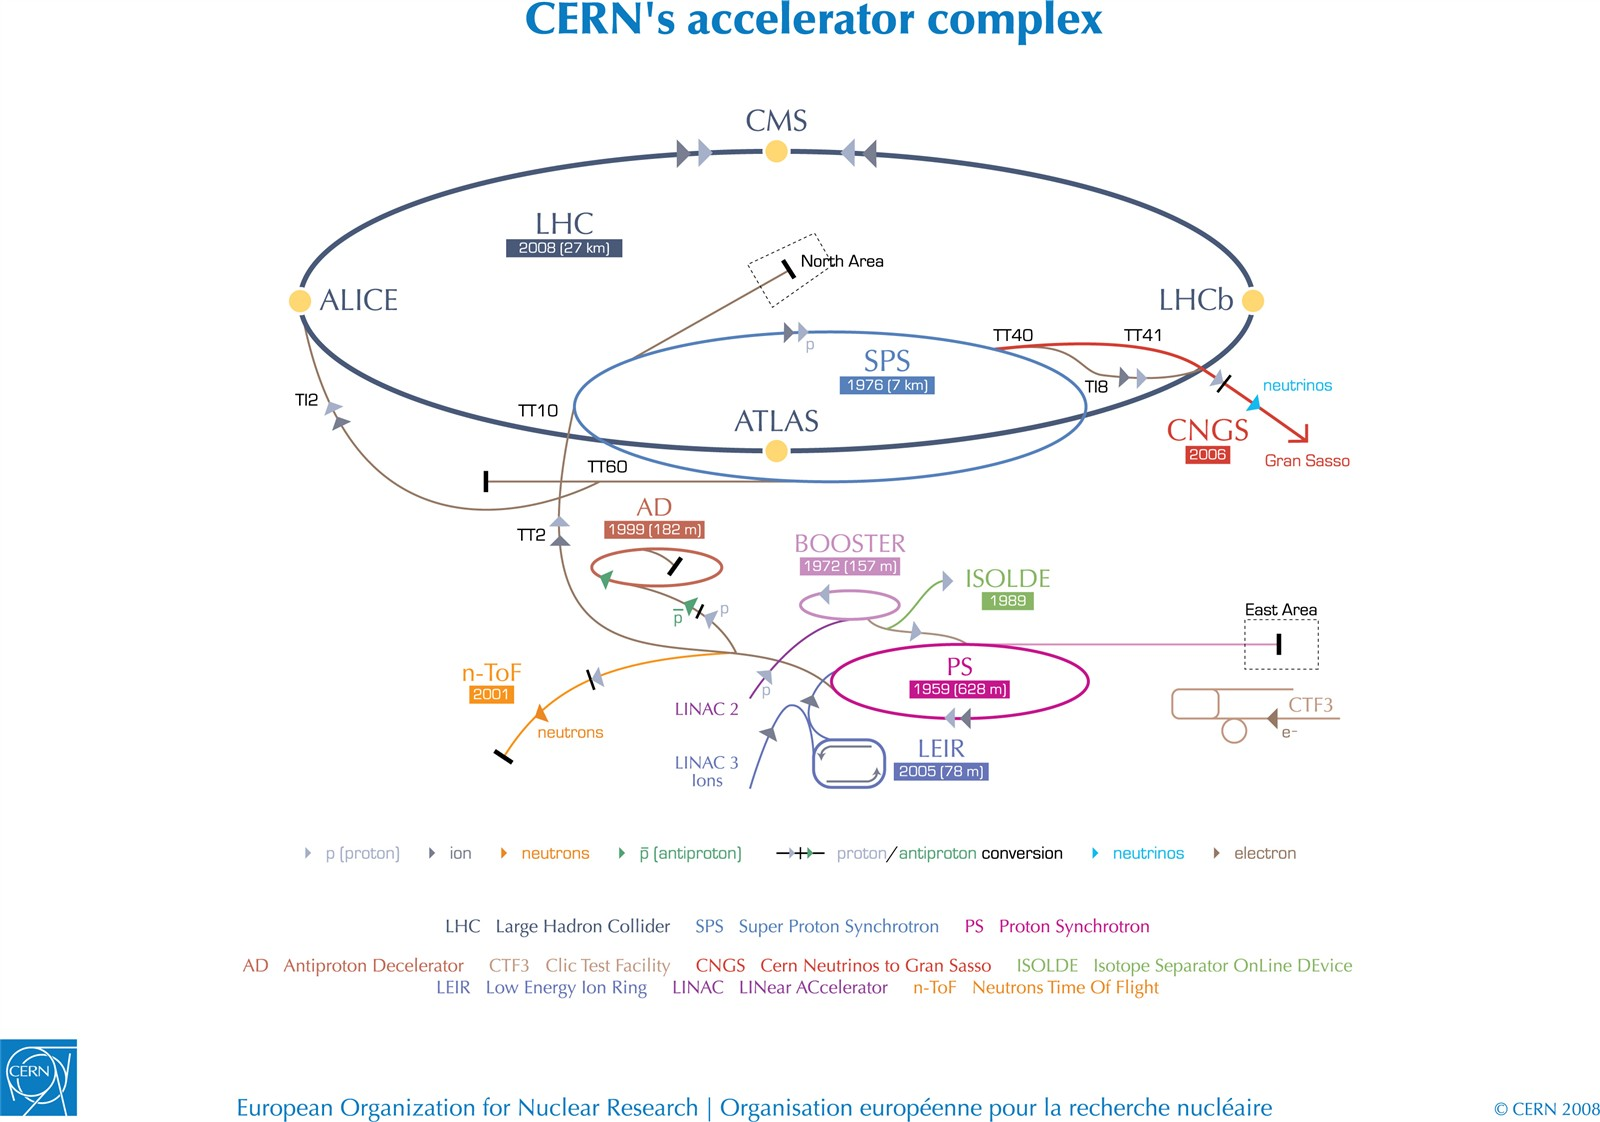
\includegraphics[width=0.95\textwidth]{Introduction/figures/cernaccelerators.jpg}
\end{center}
\caption{The CERN accelerator complex, showing both the proton and heavy ion (lead) accelerator chains from LINACs 2 and 3 up to the LHC. Different experimental uses are highlighted in the diagram.}
\label{fig:CERN-acc-complex}
\end{figure}

\section{The LHC}

The LHC is a synchrotron built to collide counter rotating beams of hadrons at an centre of mass energy of 14TeV for protons and 2.76TeV per nucleon for lead ions. It uses 1,232 superconducting dipole magnets to bend the hadron beams on a circular orbit around the beam line, in addition to using 392 quadrupole magnets for focusing in the transverse plane to maintain the bunch cross section and carry out final focusing for the 4 detector experiments in the LHC. Four detector experments are operated at the LHC; two general purpose detectors ATLAS and CMS, used for searches of new physics beyond the current energy frontier \cite{ATLASTDR,CMSDR}; LHCb, a forward detector specialised in the analysis of B-physics \cite{LHCb} and ALICE, a detector specialised in heavy ion collisions with the intent of observing the physics of quark-gluon plasma \cite{Lourenco:ALICE}. Three further experiments are in place in the LHC, LHCf (an experiment related to the effects of high-energy cosmic rays), TOTEM (measuring the total cross-section of the proton via elastic scattering processes at the collision points) and MoEDAL (an experiment searching for magnetic monopoles and stable massive particles): these three complete the experiments provided with data by collisions using LHC delivered protons.

\section{Operational Figure of Merit for a Collider - Luminosity}

One of the key figures of merit for the operation of the LHC (along with the centre of mass energy) is the luminosity at the colliding interaction regions (IRs). This is a figure which denotes the total rate of production of new (in the sense of produced during interactions during collisions between protons) particles in collider experiments. It can be thought of as the factor of proportionality between the cross section of a reaction scheme and the number of interactions per second

\begin{equation} 
\frac{dR}{dt} = \mathcal{L} \times \sigma_{p}
\end{equation}

where $\frac{dR}{dt}$ is the interaction rate. For two colliding bunches, each with a gaussian transverse distribution, the luminosity can be given in a simplified form by

\begin{equation}
\mathcal{L} = \frac{N_{1} N_{2} f_{rev} n_{b}}{4 \pi \sigma_{x} \sigma_{y}}
\end{equation}

where. Bunch populations $N_{1/2}$, the revolution frequency $f_{rev}$ and the number of bunches $n_{b}$ also contribute towards the DC beam current in the machine $I_{b} = N_{1} f_{rev} e n_{b}$. As will be seen in Sec.~\ref{sec:beam_induced_heating} the expected power loss due to beam-equipment interactions is proportional to the $I_{b}^{2}$, thus it can be seen that increasing the luminosity will increase the power loss experienced by equipment in a linear to quadratic fashion (the non-quadratic behaviour being due to other effects on the heating mechanism due to the changing beam current, explained more in Sec.~\ref{sec:beam_induced_heating}).

\subsection{Integrated Luminosity}

Following from the peak luminosity, the determinant of the quantity of experimental data is the integrated luminosity $\mathcal{L}_{int}$ is given by

\begin{equation}
\mathcal{L}_{int} = \int^{T}_{0} \mathcal{L} \left( t \right) dt
\end{equation}

where $T$ is the integrated collision time and $\mathcal{L} (t)$ is the time varying luminosity (typically decaying exponentially over the lifetime of any given fill of the collider\cite{McCrory:lumiEvo}), varying due to changing beam conditions (emittance growth) and bunch population depletion due to collisions and particle losses. The integrated luminosity is significant as the number of a given particle production schema observed by the experiments $n_{event}$ is given by

\begin{equation}
n_{event} = \mathcal{L}_{int} \times \sigma_{p}.
\end{equation}

It can thus be seen that in addition to increasing the luminosity, maximising the available time for collisions is important to maximising data collection. This requires a high level of availability of the machine, minimising failures of key systems and the down time experienced by the machine. In particular, unavoidable waiting periods between fills are to be eliminated or reduced. As is shown in Chapter~\ref{chap:mki}, long cool down times (on the order of hours, similar in magnitude to the length of the average LHC fill) for equipment that requires a specific maximum temperature to operate correctly are thus unacceptable during ideal operation and should be reduced to a minimum. These and other sources of reduction of the running time and luminosity (due to both beam coupling impedance and other sources of instabilities and interlock trips due to hardware mishaps) must thus be carefully studied and controlled by the technical and operations teams.

\section{Beam Dynamics}
\label{sec:BeamDyn}

To introduce the terms and coordinate systems used in later chapters we shall briefly introduce the some of the commonly used coordinate systems used to describe the motion of particles in circular accelerators. First we introduce the coordinate system typically used in the consideration of circular particle accelerators. Typically an ideal orbit is defined for an on momentum particle. In addition a reference frame placed upon the orbit of an ideal on-momentum particle is defined shown in Fig.~\ref{fig:accel-coord-system}. 

\begin{figure}
\begin{center}
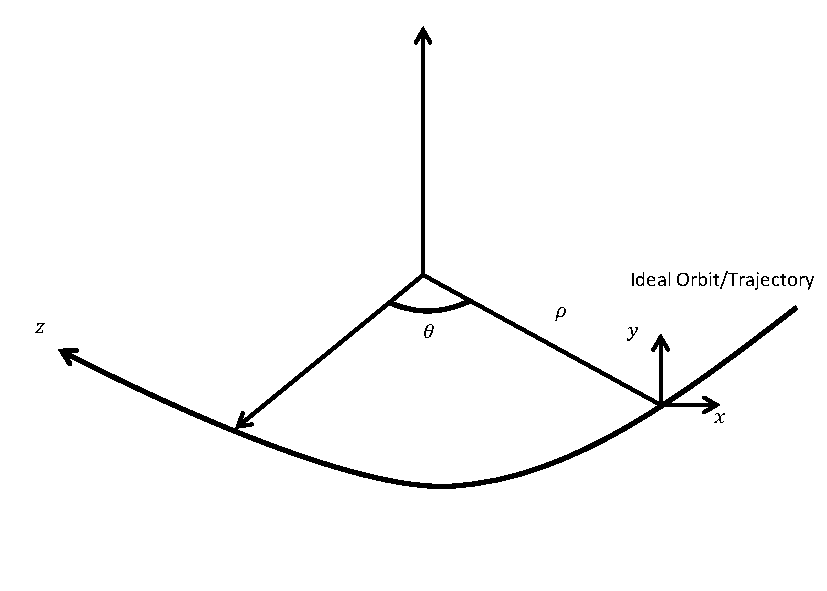
\includegraphics[width=0.75\textwidth]{Introduction/figures/coordinate-system.pdf}
\end{center}
\caption{The representation of the coordinate system of a circular accelerator, and additionally the co-moving reference frame of a circulating particle.}
\label{fig:accel-coord-system}
\end{figure}

\begin{figure}
\begin{center}
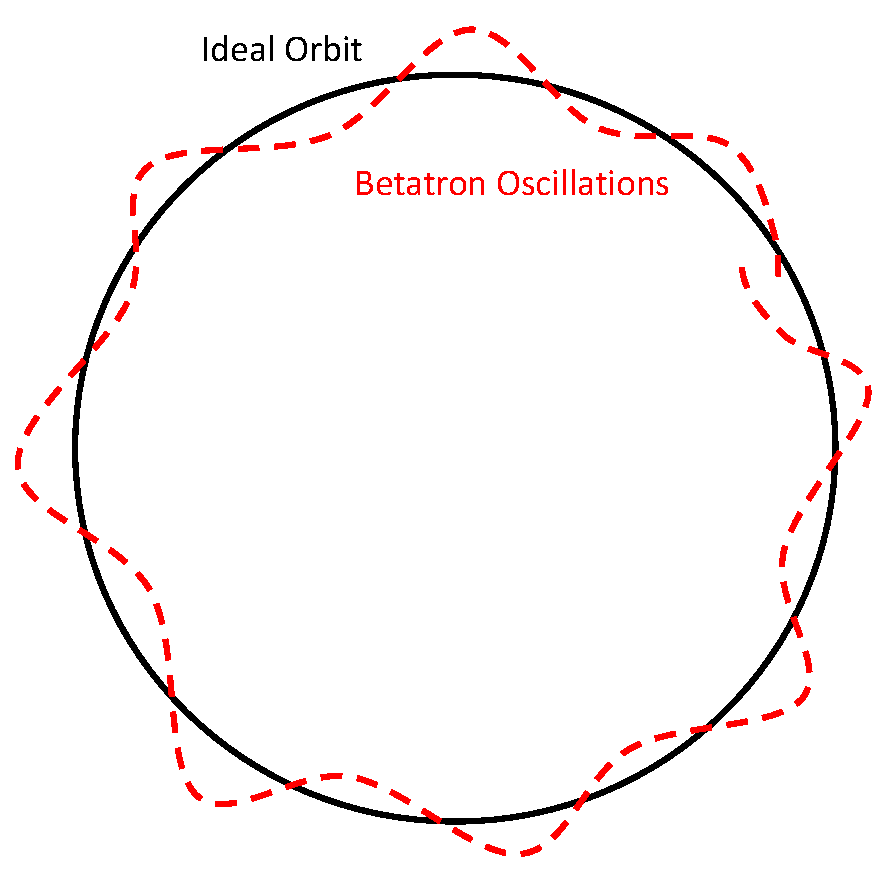
\includegraphics[width=0.65\textwidth]{Introduction/figures/betatron-motion.pdf}
\end{center}
\caption{An illustration of betatron oscillations around the ideal orbit of a circular accelerator. These oscillations occur in both the horizontal and vertical planes.}
\label{fig:betatron-motion}
\end{figure}

The use of charged particles within an accelerator is controlled by the use of both magnetic and electrical elements in the machine, leading to the particles being acted upon by the Lorentz force

\begin{equation}
\mathbf{F} = q \left( \mathbf{E} + \mathbf{v} \times \mathbf{B} \right).
\end{equation}

In high energy particle accelerators the magnetic and electric fields are typically seperated in location, with the magnetic fields only having a transverse component, being of the form

\begin{equation}
\mathbf{B} = \mathbf{\hat{x}} B_{x} + \mathbf{\hat{y}} B_{y}
\end{equation}

Due to the cross product between the velocity ($\mathbf{v} = \mathbf{\hat{z}} v$), it can be seen that there is no component of the force from the magnetic field in the $z$-direction. In addition the electric field usually only has a longitudinal component such that $\mathbf{E} = \mathbf{\hat{z}} E_{z}$. This results in the seperation of transverse and longitudinal motion such that

\begin{align}
F_{\parallel} &= qE \\
\mathbf{F_{\perp}} &= q \left( vB_{y} \mathbf{\hat{x}} - vB_{x} \mathbf{\hat{y}} \right).
\end{align}

Subsequently the transverse and longitudinal motion may both be treated independently of one another. This is discussed in detail in App.~\ref{app:BeamDyn}.

\section{Structure of Thesis}

In this thesis is studied in detail the beam coupling impedance and beam induced heating of two important devices in the LHC - the injection kicker magnets and the collimation systems, using computational simulation tools and bench-top measurement methods, and the subsequent steps taken to reduce the beam coupling impedance to reduce the heat loads on these devices. The thesis progresses as follows; we have begun by introducing the dangers of beam induced heating from the mechnical point of view, in addition to the operational figures of merit that may be limited by equipment that requires a cool down time between fills to be operated. To understand the nature of beam-induced heating, it is necessary to introduce wakefields and beam coupling impedances which are the power source for the heating. In this section we cover in some detail the beam parameters upon which beam-induced heating is dependent.

In the next chapters we introduce the tools which can be used to evaluate a structures beam coupling impedance, beam-based measurements (Chap~\ref{chap:BBmeas}), bench-top measurements (Chap.~\ref{chap:benchTopMeas}) and computational simulation tools (Chap.~\ref{chap:CompSim}). As part of this we introduce new method for evaluating the quadrupolar and constant transverse coupling impedances of asymmetric structures using the coaxial wire bench technique, verified using simulated measurements of the technique on an asymmetric structure.

In Chap.~\ref{chap:ImpRedTech} we introduce the various methods of impedance reduction, highlighting the situations in which each is appropriate, their limitations in use, and some rules of thumb for successful implementation. As part of this we carry out a study of the location of power loss in damped cavity structures with differing degreess of damping, relevant due to the relatively large losses that may occur in thermally sensitive material (i.e. ferrites) in high current machines.

In Chap.~\ref{chap:ColImp} begins the investigation of the beam coupling impedance reduction techniques as applied to a number of LHC collimation upgrades. The use of conductive coatings on the phase 2 secondary collimator jaws is discussed briefly, followed by a detailed examination of the RF screening placed in the phase 1 and phase 2-type transverse RF system, using the example of the TCTP collimator. In this case the heating is evaluated, with attention paid to the temperature of the ferrite in the phase-2 damping system to ensure that it remains an effective damping material.

In Chap.~\ref{chap:mki} the case of the beam-induced heating of the LHC injection kicker magnets is studied. The history of the observed high temperatures and the impedance reduction techniques in place is discussed. A simulation model of this complex device is made, and the simulated impedance compared to a bench-top measurements of the longitudinal and transverse impedances is made. Using the confidence given by the good agreement here, a number of alternative beam screen designs are evaluated for there longitudinal beam coupling impedance, with a constant concern for other requirements such as electrical breakdown and manufacturability.

Finally in Chap.~\ref{chap:Con} the concluding remarks are made.